\section[IB in Trees]{Information Bottleneck in Decision Trees} % Sections can be created in order to organize your presentation into discrete blocks, all sections and subsections are automatically printed in the table of contents as an overview of the talk
%------------------------------------------------
\begin{frame}
    \frametitle{Comparison: Decision Trees and Information Bottleneck Iterative Algorithm}
    
    \textbf{Common}
    \begin{itemize}
        \item Prediction: \newline
        Trees: $X \rightarrow leaf \rightarrow Y$ \newline
        IB Iterative Algorithm: $X \rightarrow \hat{X} \rightarrow Y$
        \item usage of loss function that can be expressed as expectation over $\mathbb{X}, \mathbb{Y}$ (next slide)
    \end{itemize}
    \textbf{Differences}
    \begin{itemize}
        \item IB assumes knowledge of $P_{\mathbb{X}, \mathbb{Y}}$
        \item IB requires finite $\mathcal{X}$ or explicit quantization
        \item DT is sensitive to the parameterization of $\mathbb{X}$
        \item IB finds an optimal solution, DT can and will get stuck in local optima
    \end{itemize}
\end{frame}


\begin{frame}
    \frametitle{Information Bottleneck in Decision Trees}


    $J_{IB;\beta}$ can be estimated in a decision tree:
    \begin{align*}
        J_{IB;\beta}(Y) &= I(\mathbb{X}, \hat{X}) - \beta I(\hat{X}, \mathbb{Y}) \\
        &= H(\mathbb{X}) - H(\mathbb{X}|\hat{X}) - \beta (H(\mathbb{Y}) - H(\mathbb{Y} | \hat{X})) \\
        &= const - H(\mathbb{X}|\hat{X}) + \beta H(\mathbb{Y} | \hat{X}) \\
        &= const - E_{\mathbb{X},\hat{X}}[-log P(\mathbb{X}|\hat{X})] + \beta E_{\hat{X},\mathbb{Y}}[-log(P(\mathbb{Y}|\hat{X}))] \\
        & \simeq const - 1/N \sum_i log |\{x' |x' \in X, leaf(x')=leaf(x_i)\}| \\
        &+ \beta /N \sum_i D_{KL}(y_i|| T(x_i))
        \label{eq:2}
    \end{align*}
    where $T(x)$ is the empirical distribution of $Y$ given $leaf(x)$ in the train set. \newline
    This can be greedily optimized:
    \begin{align*}
        J_{IB;\beta}(Y) &= \frac{|Y_{left}|}{|Y|} J_{IB;\beta}(Y_{left}) + \frac{|Y_{right}|}{|Y|} J_{IB;\beta}(Y_{right})
    \end{align*}
\end{frame}


\begin{frame}
    \frametitle{Information Bottleneck in Decision Trees}
    \begin{center}
        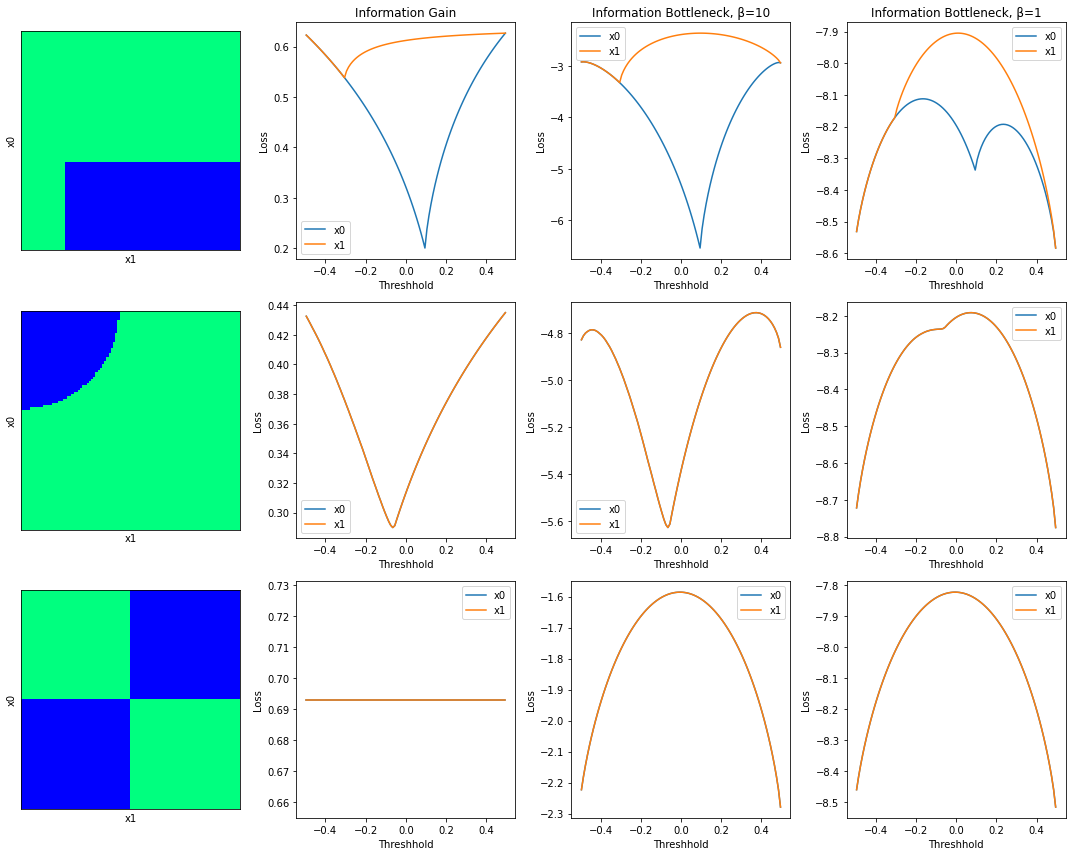
\includegraphics[width=250px]{img/optimal_split_comparison.png}
    \end{center}
\end{frame}



\begin{frame}
\frametitle{Information Bottleneck in Decision Trees}
    \begin{itemize}
        \item Similar to InformationGain + regularizer
        \item Time and space complexity of the algorithm not affected, but no more pruning necessary
        \item IB in neural networks: $I(\mathbb{X}, \hat{X})$ and $I(\hat{X}, \mathbb{Y})$ are hard to estimate
        \begin{itemize}
            \item Information Dropout \cite{achille_information_2017}: add multiplicative noise to intermediate activations
            \item MINE \cite{belghazi_mine_2018}: general purpose estimator for mututal information using neural networks, which can then be used to train another network with the IB objective
        \end{itemize}
    \end{itemize}


\end{frame}